\chapter{Implementation}
\todo{Teddy Kolla igenom detta /Teddy}
In order to achieve the project objective, it was necessary to apprehend a clear and unified understanding of how the different software components would interact with each other. The contributions made by this project is able to run alongside the existing project provided by AstaZero. To facilitate this, the application can be found in a file called ChalmersDemo.java which is an Android activity that the user of the application can decide to navigate to. The user can easily navigate between these two implementations depending on the current use-state. 
\section{Re-usability of existing software}
As mentioned before, the AstaZero team has been developing an Android application for some time that the team could utilize. The code was open source and the team decided to contribute to the existing platform instead of creating a new one. This meant that some code functions vital to the project's success already existed.

\subsection{Iso-drone}
To establish a connection with the drone, the file IsoDrone \todo{Måste jag referea till github?} provides a Java class that can be initiated to create a drone object able to communicate over the ISO22133 protocol. This meant that the team did not have to worry about the conversion of data into ISO-formatted strings but instead only could change variables of the current speed, heading, coordinates and similar and the drone object automatically transmitted this over the ISO22133 protocol. 
\\ \\
The protocol also enables the drone object to know what state ATOS is currently in and the application uses this to set up triggers for when the state changes as described in figure \ref{fig:drone-flow}

\subsection{Waypoint 1 Activity}
Since ATOS works with a local coordinate system, the location coordinates had to be converted to latitude and longitude coordinates in the Android application. This conversion was already present in the Waypoint1Activity file and works by first reducing the amount of points and then create a square matrix A with dimensions equal to the number of waypoints in the trajectory, and an array b with the same length as A's dimensions. It then populates A and b with values based on the trajectory information. Next, it uses a LUDecomposition solver to find the radii for each waypoint, which will be used to define the radius of a circular area around each waypoint in which the drone will fly.
\\

Finally, the method creates WaypointSetting objects for each waypoint in the trajectory. It uses a method to convert the waypoint's Cartesian coordinates to geographic coordinates. It then sets various properties of each WaypointSetting, including the heading, altitude, and speed of the drone at each waypoint, as well as the radius calculated earlier.

\subsection{Douglas-Peucker Algorithm} \label{douglas_puecker}
With the WaypointMission limitations presented in section \ref{sec:limit_WP}. The AstaZero team made use of the Ramer-Douglas-Peucker algorithm which is used for reducing the number of points in a curve while preserving its shape. %\todo{REFERERA!!!! http://www2.ipcku.kansai-u.ac.jp/~yasumuro/M_InfoMedia/paper/Douglas73.pdf}
This implementation made it possible to use trajectory files that normally would be composed of too many points to be run by the DJI WaypointMission software. \\  

The algorithm divides the line recursively, starting with all points between the first and last one. The first and last points are automatically selected and retained, it then identifies the point that is the maximum distance from the line segment. If the point is more than a predefined tolerance away from the line segment, it must be selected as a new start- and endpoint, otherwise the point can be discarded without impacting the shape of the curve. The algorithm recursively calls itself on the two newly created segments and the process is repeated for each new line segment until all the points are outside of the given tolerance. Figure \ref{fig:douglas_peucker} visualizes the algorithm. The result is a new curve with fewer points that still closely approximates the original one.

\begin{figure}[H]
    \centering
    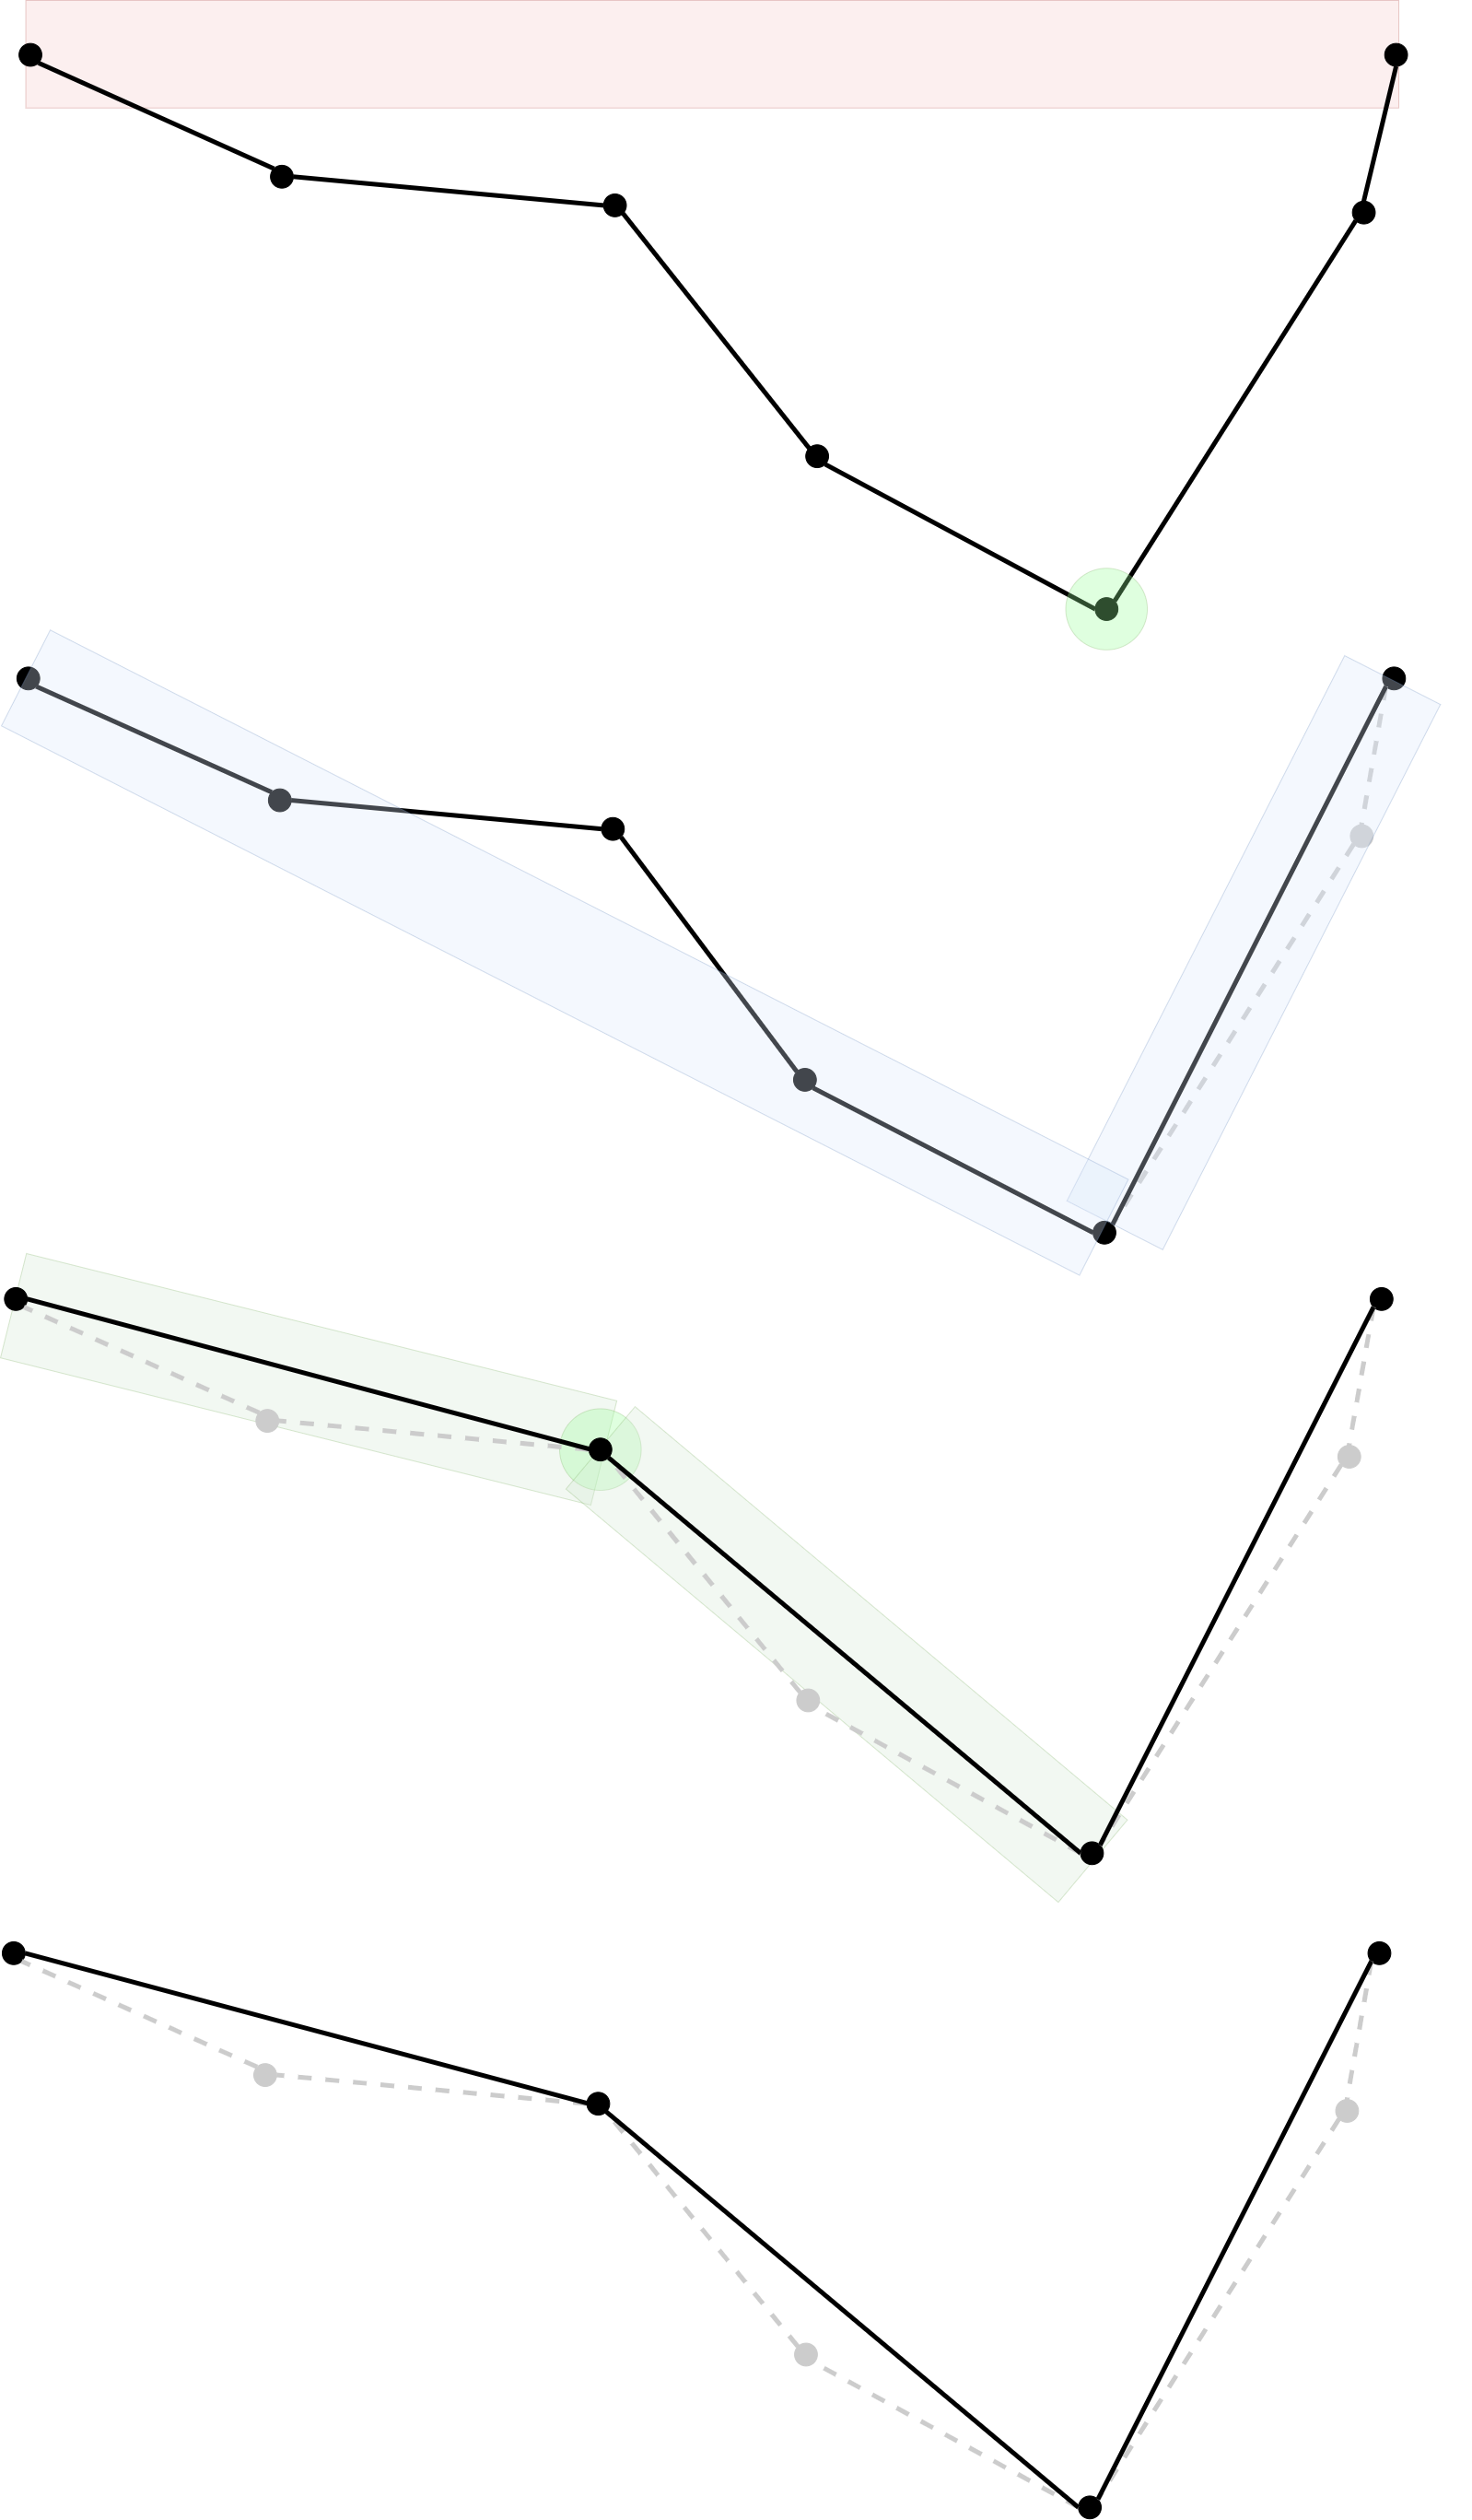
\includegraphics[scale=0.1]{figure/douglas_peucker_illustration.png}
    \caption{Illustration of the Ramer-Douglas-Peucker Algorithm}
    \label{fig:douglas_peucker}
\end{figure}
\todo{Kolla så att texten inte har massa mellanrum pga bilden}
This algorithm is heavily used when deploying curved trajectories to ISO-objects, especially drones, but it also presents a problem when deploying trajectories that only consist of points in a straight line, it reduces too many points. The solution for this problem is presented in the next section \ref{sec:alt_douglas_peucker_algo}. 

\section{Addition to Douglas-Puecker algorithm}
\label{sec:alt_douglas_peucker_algo}
The vast majority of the Douglas-Puecker implementation produced by the AstaZero team was used with only minor modification and additions. The problematic aspect of the algorithm was that it reduced too many points when presented with a trajectory in a straight line, leaving too few to points in the trajectory object to be sent to the next part of the point reduction implementation. The solution to this problem was to develop a simple collinearity check of the trajectory before applying the algorithm. If all points in the trajectories lies on a straight line the algorithm will be superseded as it is overly complex for such a simple case. 
\newline

The addition to the algorithm works by extracting the two first point of the input in order to create a reference line for all remaining points. It then makes use of one of the algorithms loops which iterates through every point in the input, if the cross product of resulting vector from the first to the current point and the reference line is zero, the current point is collinear with the reference line. This calculation is done for every point in the input trajectory and if any resulting vector from the current point would fail to produce a cross product equal to zero, a \textit{isCollinear} variable would be set to false. This would disable the superseding of the Douglas-Puecker algorithm and allow to to run as intended. Algorithm \ref{DP_code} describes the addition to the Douglas-Puecker algorithm in pseudocode. 

\begin{algorithm}[H] \label{DP_code}
\caption{Pseudo code of the addition to the existing Douglas-Peucker algorithm}
\SetAlgoLined
\SetKwFunction{douglasPuecker}{doglasPuecker}
\SetKwProg{Fn}{Function}{:}{}
\Fn{\douglasPuecker{$traj$, $resultTraj$}}{
$**Algorithm\ starts**$

\If{size of $traj$ < 3}{
\Return $traj$
}
$isColinear \gets true$;

$x1, y1 \gets traj[0]$;

$x2, y2 \gets traj[size\ of\ traj]$;

\For{$i$ \gets 0\ \KwTo\ size\ of\ traj}{
$...$

$px, py \gets traj[i]$;
$crossProduct \gets (x2 - x1) \cdot (py - y1) - (y2 - y1) \cdot (px - x1)$;

\If{$crossProduct \neq 0$}{
$isColinear \gets false$;
}

$...$
}

\If{size of $traj$ > max number of points \& isColinear}{
$multiplier \gets \lfloor \frac{\text{size of } traj}{\text{max number of points}}\rfloor$;

\For{$i\gets 0$ \KwTo size of $traj$-1}{
$resultTraj \gets resultTraj + [traj[i]]$;

$i \gets i + multiplier$
}
$resultTraj \gets resultTraj + traj[size\ of\ traj]$;

\Return $resultTraj$;
}
%\caption{Collinearity addition to Douglas-Peucker algorithm}
}
\end{algorithm}

\section{Chalmers Demo Activity} \label{sec:chalmers_demo_activity}


Activities serve as the fundamental building blocks of any Android application, including the application provided by AstaZero. Each activity corresponds to a distinct screen within the application, serving as the primary element responsible for displaying and managing the graphical user interface. The GUI is then be comprised of many different elements, such as buttons, text views, images, and input fields, and can interact with other activities, components and code. The provided application consisted of several activities with its own GUI, that managed their own tasks, such as making sure the remote controller has a connection to a drone. The first iteration of the Chalmers Demo Activity GUI is presented in the next section, \ref{sec:implement_GUI}. 



\section{Graphical user interface} \label{sec:implement_GUI}
The GUI was developed continuously during the course of the project, going through different iterations. The goal with the GUI was to make it as easy and as intuitive as possible, limiting the amount of buttons and information shown on the screen. The information relevant was determined to be:
\begin{itemize}
    \item The video feed of the camera with detected objects highlighted
    \item Latitude, longitude and altitude
    \item Drone state
    \item Mission information
    \item IP address of the phone
    \item Buttons for starting, stopping, landing and resetting the missions
\end{itemize}
%%https://developer.android.com/develop/ui/views/layout/relative
\begin{figure}[!h]
    \centering
    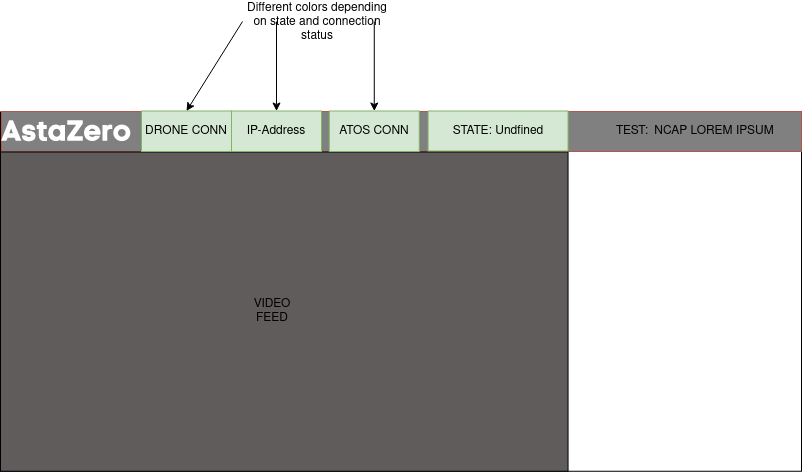
\includegraphics[width=\textwidth]{figure/v_1.2_GUI_demo_app.png}
    \caption{The first design idea for the GUI}
    \label{fig:my_label}
\end{figure}
This was implemented using the programming language XML and relies on a RelativeLayout hierarchy\todo{ref} and contains different views. 
\newline

While the drone control application has yet to be finalized, the GUI implementation has come a long way. The initial plan was to create two separate applications - one for image recognition and another for sending trajectory data to the drone - the first version of the application was developed to implement these functions separately. This was quickly merged in to one development process and went through some iterations, but kept the general layout. The goal remained the same, to make it as simple and easy to use as possible. The team added and removed parts as the team gathered more knowledge and information from the client during the project.


\section{DJI Flight Controller} \label{sec:DJI_flight_controll}
The flight aspect of the project is one of two main parts, the other one being object tracking presented in section \ref{sec:object_track}.

\subsection{Updating the flight controller}
As presented in section \ref{Java, Android....} the Android application makes heavy use of DJI's mobile SDK as it is the primary way of for third party software to interact with the drone. The foundation of this interaction is built upon the flight controller object, it facilitates the interaction between the drone's different flight enabling systems. 
\newline

The flight controller is initialized via its DJI SDK constructor, this is also where a callback state for the controller is specified. On every update, which is set to be initiated 10 times every second, the callback provides the program with relevant information, such as of the drone's GPS position in latitudinal and longitudinal coordinates, strength of the GPS signal and the current altitude. During the callback, the method which update the flight data is called. In this method, the flight controller object is then utilized multiple times in several different methods. The primary use involves creation, deployment and activation of the WaypointMissions. The update flight data is also the part which integrates ATOS into the android application, figure \ref{fig:drone-flow} and the following paragraph describes the integration. 

\begin{figure}[H]
    \centering
    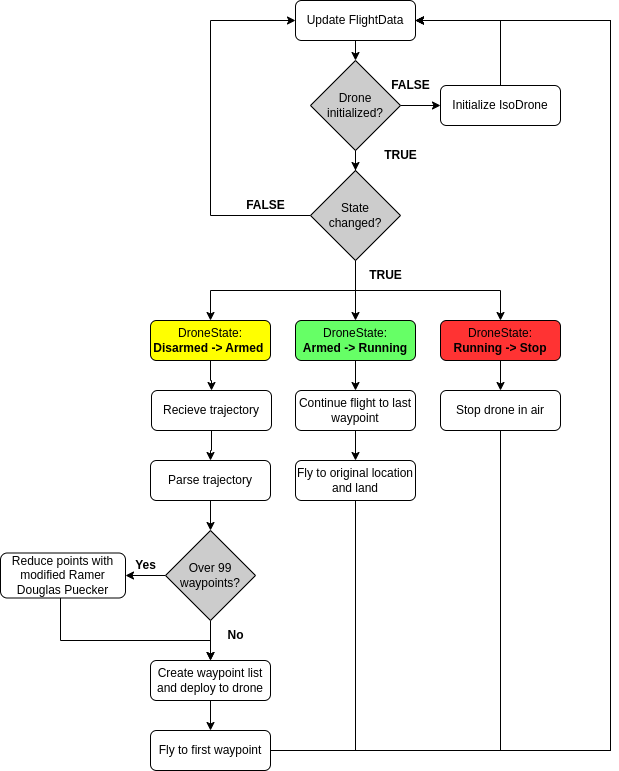
\includegraphics[scale=0.5]{figure/Flowchart-drone.png}
    \caption{Flight data update flow chart}
    \label{fig:drone-flow}
\end{figure}

ATOS makes use of a object control module that communicates and sends transmission of trajectories via the ISO22133 protocol for all ISO-objects in the current test. The drone application subsequently receives this data through its corresponding ISO-drone object when ATOS cycles states, this prompts the flight data to be updated and different sequences of actions are triggered.
\newline

When the state of the ISO-drone changes from Disarmed to Armed, the trajectory is passed through the application and verified that its in the right format. If the trajectory is too large, it is to be reduced by the algorithm described in sections \ref{douglas_puecker} and \ref{sec:alt_douglas_peucker_algo}. When the trajectory is correct, the application transforms the trajectory into global latitudinal and longitudinal coordinates through a coordinate conversion script developed by AstaZero. The application then transmits the trajectories to the drone via a DJI protocol from the remote controller connected the the android phone. Following this, the test commences when the ATOS state is changed to "Running", and the drone as well as all other test objects execute their pre-determined paths. 

\subsection{Updating the GUI} \label{sec:updating_UI}

Updating the user interface is crucial for providing real-time information about the drone's location, altitude, and GPS signal strength as well as showing the test track personnel what is currently being filmed. The GUI must be updated continuously, and this is achieved by also sending information to the GUI when receiving the callback presented in section \ref{sec:flight_controll}. The GUI also utilized information such as IP-address and ATOS state from the ISO-drone object as well as which the target waypoint in the current WaypointMIssion from the flight controller. 



\section{Image recognition} \label{sec:image_rec}
As mentioned in 2.2.7 TensorFlow Lite will be used for object detection in the project mainly because it has the fast response that is needed during the test. The image recognition is heavily inspired by an open source project \todo{Github källan: https://github.com/mrinalTheCoder/ObjectDetectionApp} that have already done a object detection application using Tensorflow Lite. 
\\ \\
The pre trained model that is used is trained to detect 90 objects such as a person, car, bicycle and some more objects. A reason a model that can detect 90 objects is used is due to that it is more reliable than a model that is trained to only detect 2 objects like a person and car, which is mostly used during a Euro NCAP test. That is because if a model could only detect a person and a car it more often than not label a object as something that it isn't. Another reason that this model is used is because it can detect objects such as trucks, motorcycles, buses and more objects that could potentially be used during tests. The problem that could occur when using a bigger model is that it is slow but testing the model in action it responded fast enough. \todo{Axel, skriv lite om hur modelen fungerar med coco och ssd}
\\ \\
The camera feed from the phone is sent to the application in a RAW format and shown on the screen. After the video is shown, a frame from the feed is sent to run in the background to be converted from RAW to RGBA in a bitmap format due to that is how the frame needs to be in order for it to run through the model. When the frame is in the right format it is being sent to run through the object detection. The output you get from that are the following:
\begin{enumerate}
    \item Index - all the objects is numerated
    \item Labels - what kind of object is it
    \item Confidence - How sure the model is about the predicted object from 0-100 \%
    \item Rectangle - A rectangle over the objects location
\end{enumerate}
Since the interesting objects in this case is people and cars the detection function has been modified to only send the data about those objects who have been labeled person or car. To be more confident that the model doesn't label a object as something that it isn't the function check if the confidence is over 50\% then the object is valid. When done running through the frame and labeling the objects the rectangles for each object will be presented on the screen as an overlay view over the video feed. To the rectangles it is also shown what the label for the object is and what the confidence is.

\begin{figure}[H]
    \centering
    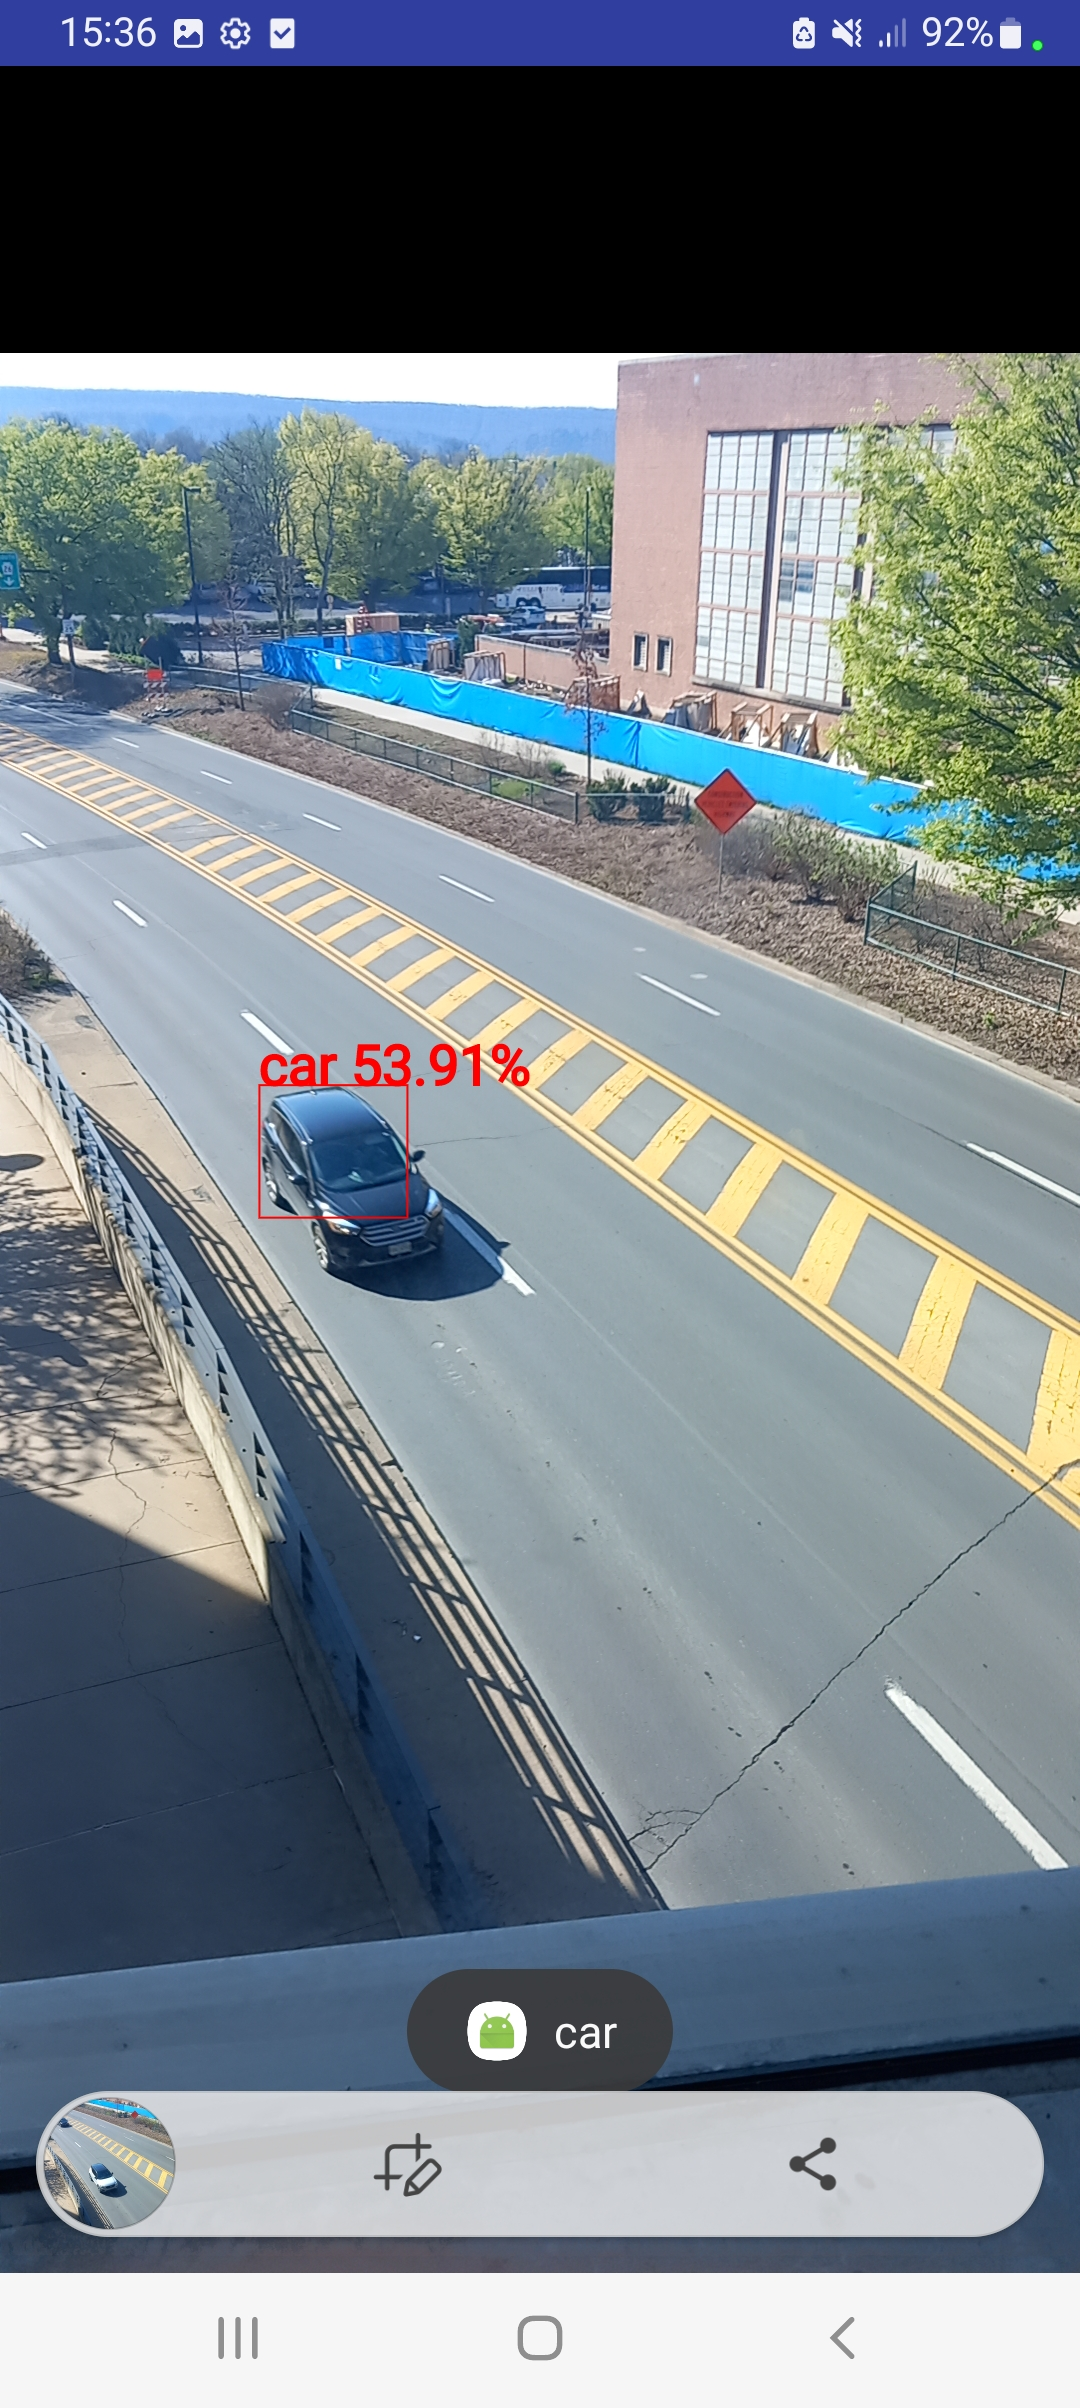
\includegraphics[scale=0.15]{figure/ObjectDetection_car.jpg}
    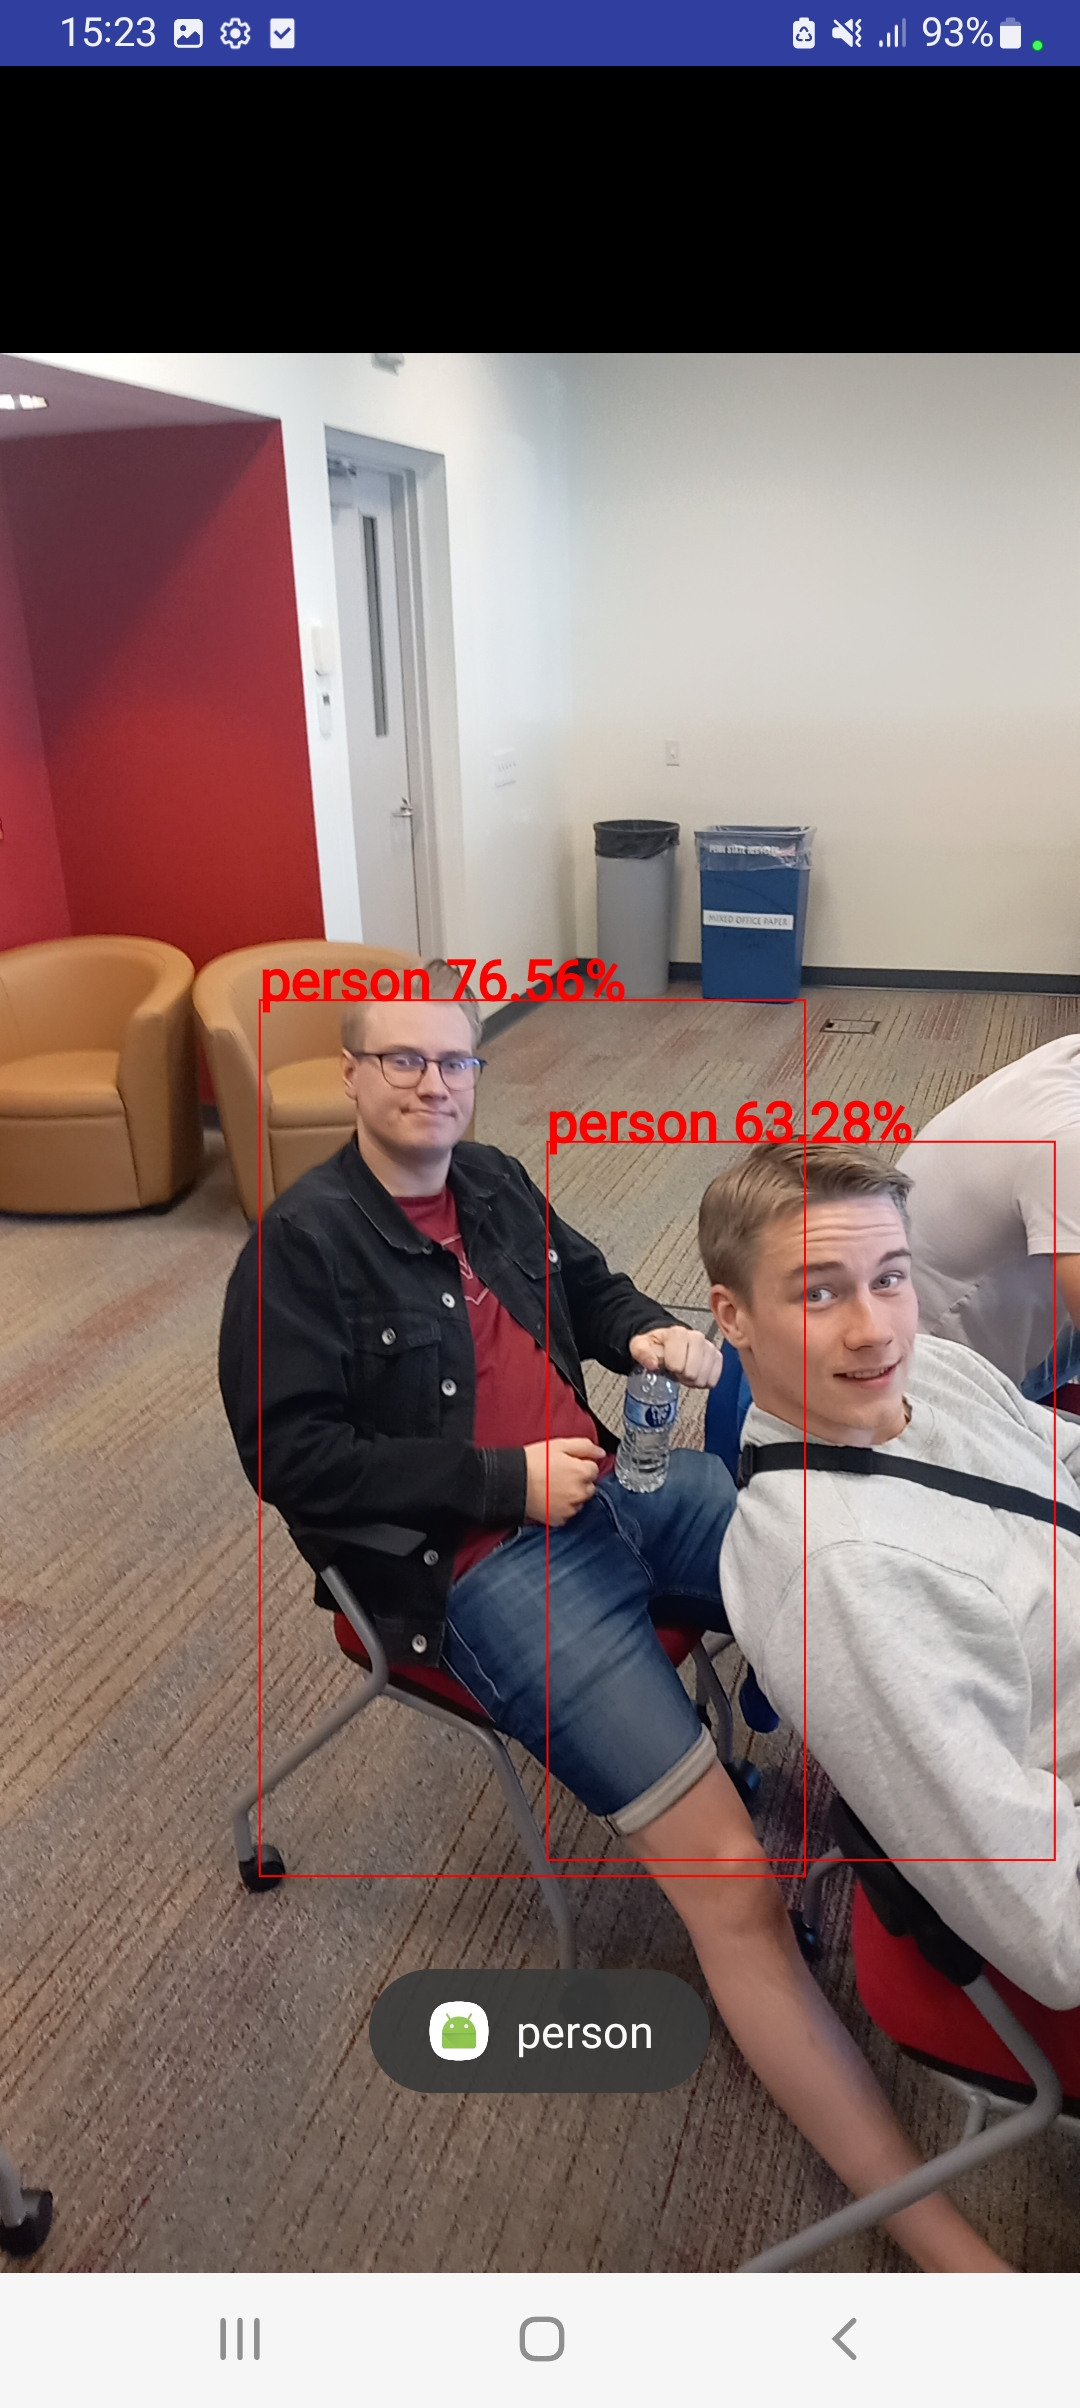
\includegraphics[scale=0.15]{figure/ObjectDetection_person.jpg}
    \caption{Screenshots from the phone}
    \label{fig:Objectdetection-screenshot}
\end{figure}




%To use Tensorflow Lite the application firstly needs to take in a frame from the video feed in a Bitmap format. To achieve this there needs to be some sort of callback to receive the frame data to run the image through the model. In this case the gimbal is sending the video in the format of H.264 but DJI SDK offers a YUV data callback solution which make it possible to receive a frame from the video feed but now in the YUV data format. \todo{lägg in källa: https://developer.dji.com/api-reference/android-api/Components/CodecManager/DJICodecManager.html}. When the receiver gets the frame in the YUV data format there needs to be a transformation to make the YUV into a Bitmap. \todo{Ska vi prata om alla problem som uppstod med DJI SDK som gjorde att vi inte blev klara eller förklara vad som hade hänt om DJI inte är några rövhål?}

\section{Object tracking} \label{sec:object_track}
\todo{Fundera på om det ska skrivas något här/JG}






% \subsection{Merging the apps}
% When both apps worked decently we tried merging the apps. Pretty quickly we realized the DJI SDK did not support running parallel missions in our case the waypoint mission and the activetrack mission. We are currently working on fixing this, by using the waypoint mission and running a convolutional neural network to identify cars on images from the video feed then using the pixel-coordinates of the object to adjust the gimbal.

